\documentclass[12pt, oneside]{article}
\usepackage[letterpaper, margin=1in, headsep=0.5in]{geometry}
\usepackage[english]{babel}
\usepackage[utf8]{inputenc}
\usepackage{amsmath}
\usepackage{amsfonts}
\usepackage{amssymb}
\usepackage{tikz}
\usetikzlibrary{quotes, angles}
\usepackage{graphicx}
%\usepackage{pgfplots}
%\pgfplotsset{width=10cm,compat=1.9}
%\usepgfplotslibrary{statistics}
%\usepackage{pgfplotstable}
%\usepackage{tkz-fct}
%\usepackage{venndiagram}

\usepackage{fancyhdr}
\pagestyle{fancy}
\fancyhf{}
\rhead{\thepage \\Name: \hspace{1.5in}.\\}
\lhead{BECA / Dr. Huson / Geometry 10th Grade\\* Unit 1: Introduction to Geometry\\5 October 2018}

\renewcommand{\headrulewidth}{0pt}

\begin{document}
\subsubsection*{Exam 1b: Angle Pairs}
  \vspace{0.5cm}
  \begin{enumerate}

  \item Complete the construction of an angle bisector including the six steps.
    \begin{enumerate}
      \item Given an angle with vertex $A$.
      \item Construct circle $A$ with arbitrary radius (i.e. the radius does not matter).
      \item Label the intersections $B$ and $C$ of the angle's rays and circle $A$.
      \item Construct circle $B$  with radius $BC$. \bigskip
      \item Construct circle $\rule{2cm}{0.15mm}$  with radius $\rule{2cm}{0.15mm}$. \bigskip
      \item Label $D$, the intersection of circle $B$ and $C$. \bigskip
      \item Draw ray $\rule{2cm}{0.15mm}$.
      \bigskip
      \item Ray $\overrightarrow {AD}$ bisects $\angle A$.
    \end{enumerate}
    \vspace{3cm}
    \begin{center}
    \begin{tikzpicture}
      \draw [<->, thick] (5,6)--(0,0)--(9,0);
      \draw [fill] (0,0) circle [radius=0.05] node[below]{$A$};
      %\draw [fill] (7,0) circle [radius=0.05] node[below]{$N$};
    \end{tikzpicture}
    \end{center}
\newpage

  \item Complete the construction of a perpendicular bisector including the six steps.
    \begin{enumerate}
      \item Given the line segment $\overline{PQ}$.
      \bigskip
      \item %Construct circle $P$ with radius $\rule{2cm}{0.15mm}$.
      \bigskip
      \item %Construct circle $\rule{2cm}{0.15mm}$  with radius $\rule{2cm}{0.15mm}$.
      \bigskip
      \item %Label the intersection $P$ of the two circles.
      \bigskip
      \item Draw the line $\rule{2cm}{0.15mm}$.
      \bigskip
      \item The line $\rule{2cm}{0.15mm}$ is the perpendicular bisector of $\overline{PQ}$.
    \end{enumerate}
    \vspace{7cm}
    \begin{center}
    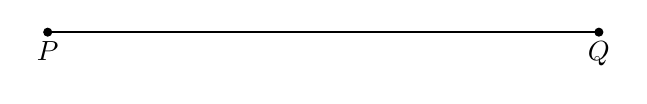
\begin{tikzpicture}
      \draw [-, thick] (0,0)--(7,0);
      \draw [fill] (0,0) circle [radius=0.05] node[below]{$P$};
      \draw [fill] (7,0) circle [radius=0.05] node[below]{$Q$};
    \end{tikzpicture}
    \end{center}
\newpage



  \end{enumerate}

\end{document}
